\section{卷积神经网络}
\subsection{卷积神经网络概述}
卷积神经网络的特点在于能够提取出一个图像中的各种特征。其原理为自然图像的一
部分的统计特性与其他部分是一样的。也就是说在这一部分学习的特征也能用在另一部分
上,所以对于这个图像上的所有位置,我们都能使用同样的学习特征(权值)。
我们提取一种特征用一种卷积核,卷积核为下图左边图像黄色部分,卷积核的权值为
黄色部分右下红色字体。
\begin{center}
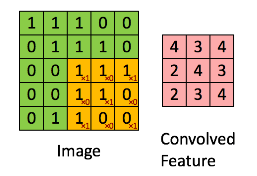
\includegraphics[scale=0.7]{../figures/conv.png} 
\end{center}
设大矩阵的大小为为$d\times d$,利用大小为$m\times m$的卷积核可以得到特征提取
降维后的大小为$(d-m+1)\times(d-m+1)$的矩阵。这个过程为一个特征的提取。在卷积
的过程中,从原图像(Image)矩阵$I$生成的卷积特征矩阵$C$(Convolved Feature)中的
每个元素为:
\begin{eqnarray}
C_{ij}=\sum_{u=1}^m\sum_{v=1}^mw_{uv}I_{i+u-1,j+v-1}
\end{eqnarray}
其中,$i,j\in(d-m+1)$
对于卷积特征矩阵(Convolved feature)我们下一步进行池化。池化的目的是对图像
不同位置进行聚合统计来描述大的图像。聚合统计可以通过计算一个区域上某个特定特征
的平均值或者最大值,这样可以降低更多的维度以及不容易过拟合。如果选择图像中连续
的范围作为池化区域,并且只是池化重复的隐藏单元产生的特征,那么这些池化单元具有
平移不变性。这就意味着即使图像经历了一个小的平移之后依然会产生相同的池化特征。
池化过程如下图:
\begin{center}
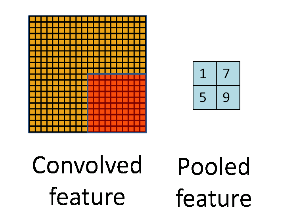
\includegraphics[scale=0.7]{../figures/pool.png} 
\end{center}
我们叫上图左图红色部分为一个池,并且通常取能够将卷积特征矩阵平均划分的大小的池。
池化后我们得到池化特征矩阵$P$(Pooled feature),我们设卷积特征图像为长宽都为$c$的
矩阵,则池长宽设为$p$,若为最大池化则$P$的元素为:
\begin{equation}
P_{ij}=\max_{u\in[1,p],v\in[1,p]}\{C_{u+(i-1)\times(p+1),v+(j-1)\times(p+1)}\}
\end{equation}
其中,$i,j\in[1,\frac{c}{p}]$。
若采用平均池化,则$P$的元素为
\begin{eqnarray}
P_{ij}=\frac{1}{p^2}\sum_{v=1}^p\sum_{u=1}^pC_{u+(i-1)\times(p+1),v+(j-1)\times(p+1)}
\end{eqnarray}
其中,$i,j\in[1,\frac{c}{p}]$。事实上,在设置卷积核时,一般将其设置为四维,各个维度分别为:卷积核长、卷积核宽、上一层的图像深度,卷积核个数。另外,对于一些深度学习的任务,是需要重复卷积很多次,为了实现这一目的,需要确保卷积之后图像长宽不变,于是在卷积之前通常在图像周围补足够个数的0,以扩大图像的尺寸,使得卷积之后的图像与原来的图像尺寸相同。

卷积神经网络其实可以包含两个大的部分,分别为特征提取层与分类器层。特征提取层包含若干个卷积层和池化层。在特征提取层中,只需要训练卷积层,而卷积层的共享参数与卷积核的属性,相比于全连接神经网络,参数更少,且抓住了图像的特征。特征提取层的输出需要转化之后,才能接入分类器层,一般的做法是将输出拉长为向量,而分类器层一般是用全连接的神经网络,最后接入softmax层,与标签计算损失函数,进而反向传播。下图是一种卷积网络结构,其对应的任务是手写数字识别。

\begin{center}
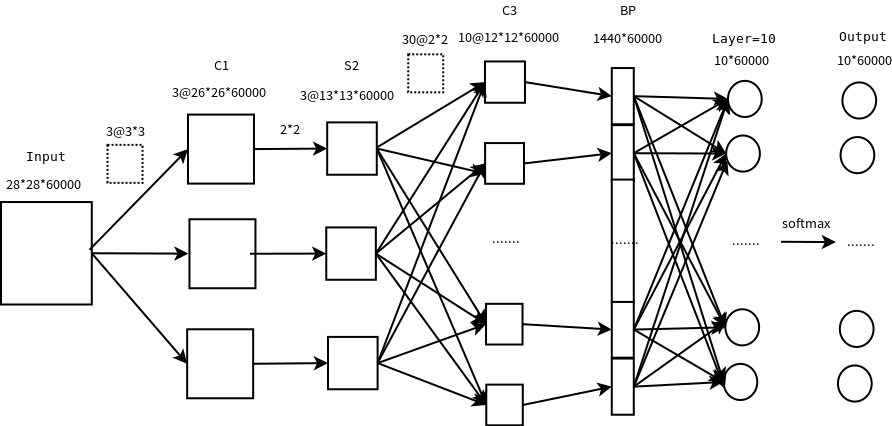
\includegraphics[scale=0.4]{../figures/CNN1.png} 
\end{center}
\subsection{经典CNN模型}
\paragraph{AlexNet}AlexNet结构上由8层隐含层组成,前五层为特征提取层,后三层为分类器层,用于做图像分类。其具体的结构如下:
\begin{center}
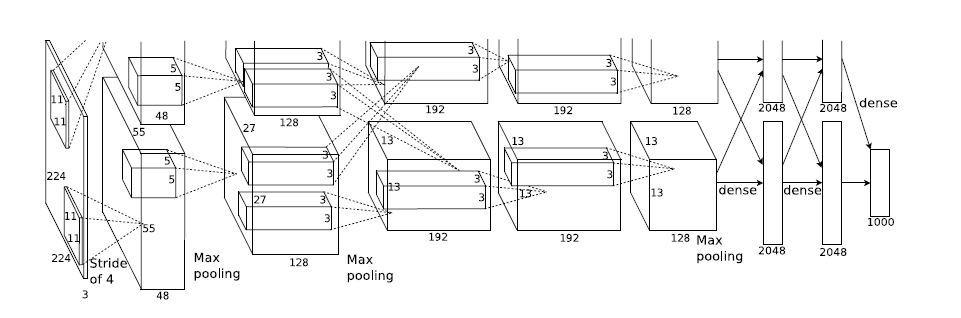
\includegraphics[scale=0.6]{../figures/AlexNet.png} \\
AlexNet结构,需注意的是,隐含层计算时分为上下部分计算,实际上是一个分布式计算的想法。
\end{center}
AlexNet当年提出来用已解决ImageNet的分类问题,对于$224\times224$像素的三通道照片,第一层使用$11\times11\times3\times96$的卷积核;第二层使用$5\times5\times96\times256$的卷积核,并进行最大池化;第三层使用$3\times3\times256\times384$的卷积核;第四层使用$3\times3\times384\times384$的卷积核;第五层使用$3\times3\times384\times256$的卷积核;之后连接全连接层,第六、七层都为4096个神经元,第八层则使用softmax。AlexNet的创新点在于激活函数采用了ReLU与dropout。
\paragraph{VGGNets}
\subsection{迁移学习}
\subsection{CNN+}



\subsection{Batch Normalization}


